\newpage
\section{La Loi Normale (ou Gaussienne)}

\subsection{Introduction et Fonction de Densité (PDF)}

Après les lois discrètes et les lois continues de base (Uniforme, Exponentielle), nous abordons la distribution la plus célèbre et la plus utilisée en probabilités et statistiques.

\begin{definitionbox}[Loi Normale]
Une variable aléatoire continue $X$ suit une \textbf{loi normale} (ou loi de Gauss) de paramètres $\mu$ (l'espérance) et $\sigma^2$ (la variance), notée $X \sim \mathcal{N}(\mu, \sigma^2)$, si sa fonction de densité de probabilité (PDF) est donnée par :
$$ f(x; \mu, \sigma) = \frac{1}{\sigma \sqrt{2\pi}} e^{ -\frac{1}{2} \left( \frac{x-\mu}{\sigma} \right)^2 } $$
pour tout $x \in (-\infty, \infty)$, où $\sigma > 0$.
\end{definitionbox}

Cette formule, bien qu'imposante, décrit une forme très familière : la courbe en cloche.

\begin{intuitionbox}[La Courbe en Cloche]
La loi normale est sans doute la distribution la plus importante en probabilités et statistiques. Pourquoi ? Parce qu'elle modélise remarquablement bien de nombreux phénomènes naturels et processus aléatoires où les valeurs tendent à se regrouper autour d'une moyenne, avec des écarts symétriques devenant de plus en plus rares à mesure qu'on s'éloigne de cette moyenne. Pensez à la taille des individus dans une population, aux erreurs de mesure répétées, ou même aux notes d'un grand groupe d'étudiants à un examen bien conçu. 

Sa densité a une forme caractéristique de \textbf{cloche symétrique} :
\begin{itemize}
    \item \textbf{Le Centre ($\mu$)} : Le paramètre $\mu$ représente l'\textbf{espérance} (la moyenne) de la distribution. C'est le centre de symétrie de la courbe, là où la cloche atteint son \textbf{sommet}. C'est la valeur la plus probable (le mode) et aussi la valeur qui coupe la distribution en deux moitiés égales (la médiane). Changer $\mu$ \textit{translate} la cloche horizontalement sans changer sa forme.
    \item \textbf{La Dispersion ($\sigma$)} : Le paramètre $\sigma$ est l'\textbf{écart-type} ($\sigma^2$ est la variance). Il mesure la \textbf{dispersion} des valeurs autour de la moyenne $\mu$. Géométriquement, $\sigma$ contrôle la \textbf{largeur} de la cloche.
        \begin{itemize}
            \item Un \textit{petit} $\sigma$ signifie que les données sont très concentrées autour de la moyenne, donnant une cloche \textbf{étroite et pointue}.
            \item Un \textit{grand} $\sigma$ signifie que les données sont plus étalées, donnant une cloche \textbf{large et aplatie}.
        \end{itemize}
    Les points d'inflexion de la courbe (là où la courbure change de sens) se situent exactement à $\mu \pm \sigma$.
\end{itemize}

\tcblower
\centering
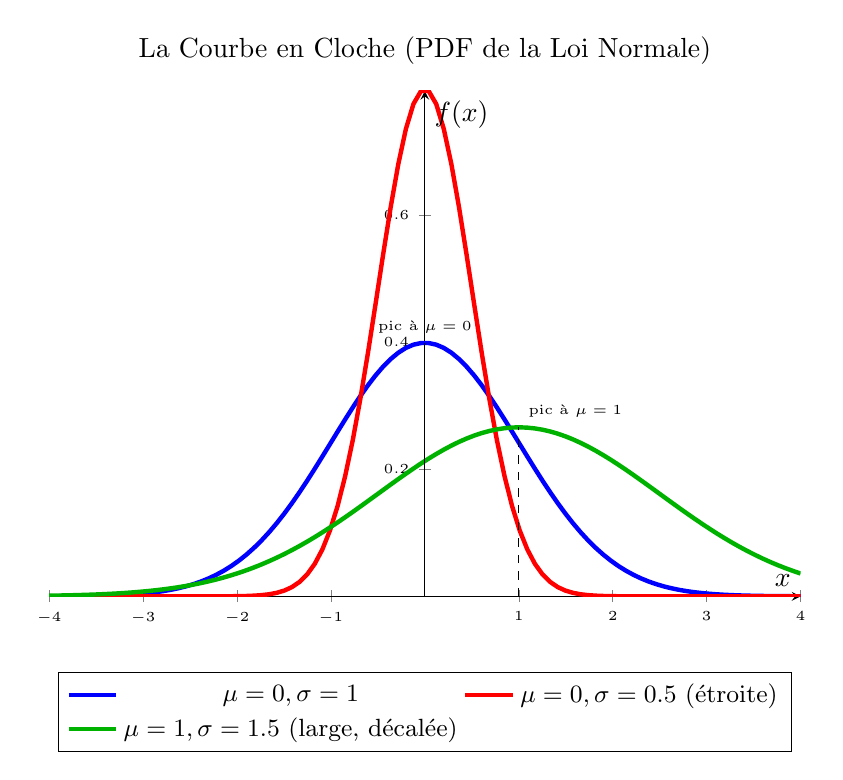
\begin{tikzpicture}
    \begin{axis}[
        title={La Courbe en Cloche (PDF de la Loi Normale)},
        xlabel={$x$},
        ylabel={$f(x)$},
        axis lines=middle,
        no markers,
        samples=100,
        domain=-4:4,
        height=8cm,
        width=\linewidth-1cm,
        tick label style={font=\tiny},
        legend style={at={(0.5,-0.15)}, anchor=north, font=\small},
        legend columns=2
    ]
    % N(0, 1)
    \addplot [blue, ultra thick] {1/(sqrt(2*pi))*exp(-x^2/2)};
    \addlegendentry{$\mu=0, \sigma=1$};
    % N(0, 0.25) => sigma=0.5
    \addplot [red, ultra thick] {1/(0.5*sqrt(2*pi))*exp(-x^2/(2*0.5^2))};
    \addlegendentry{$\mu=0, \sigma=0.5$ (étroite)};
    % N(1, 2.25) => sigma=1.5
    \addplot [green!70!black, ultra thick] {1/(1.5*sqrt(2*pi))*exp(-(x-1)^2/(2*1.5^2))};
    \addlegendentry{$\mu=1, \sigma=1.5$ (large, décalée)};

    \draw [dashed] (axis cs:0,0) -- (axis cs:0, {1/(sqrt(2*pi))}) node[above, font=\tiny] {pic à $\mu=0$}; % Ligne pour mu=0
    \draw [dashed] (axis cs:1,0) -- (axis cs:1, {1/(1.5*sqrt(2*pi))}) node[above right, font=\tiny] {pic à $\mu=1$}; % Ligne pour mu=1
    \end{axis}
\end{tikzpicture}
\par\small\textit{Influence de $\mu$ (position) et $\sigma$ (largeur) sur la forme de la cloche.}
\end{intuitionbox}

Mais d'où vient cette formule spécifique ? Il existe une dérivation fascinante à partir d'hypothèses fondamentales sur les erreurs aléatoires (argument d'Herschel-Maxwell).

\begin{proofbox}[Dérivation de la Densité Normale à partir des Principes Fondamentaux]

\textbf{Contexte Visuel :} Imaginons un nuage de points dispersés autour d'une cible à l'origine $(0,0)$, comme des impacts de fléchettes. Le graphique ci-dessous illustre cette dispersion. On s'intéresse à la probabilité de tomber dans une petite zone, comme $dA$, autour d'un point $(x, y)$.

\begin{center}
\begin{tikzpicture}
\begin{axis}[
    axis lines=middle, % Axes qui passent par l'origine (0,0)
    xlabel=$x$,       % Étiquette axe X
    ylabel=$y$,       % Étiquette axe Y
    axis line style={magenta}, % Couleur des axes
    xlabel style={anchor=west, magenta}, % Style de l'étiquette X
    ylabel style={anchor=south, magenta}, % Style de l'étiquette Y
    xmin=-3.5, xmax=3.5, % Limites du graphique
    ymin=-3.5, ymax=3.5,
    tick label style={font=\tiny} % Police plus petite pour les graduations
]

% Ajout des points du nuage. Ce sont des coordonnées approximatives.
\addplot [only marks, mark=*, cyan, mark size=1.5pt]
coordinates {
    (0.2, 0.1) (-0.5, 0.2) (0.1, -0.3) (0.5, -0.8) (-0.3, -1.2) (0,0.1)
    (1.5, 1.5) (0.8, 0.8) (2.0, -0.5) (2.8, -1.4) (2.5, -0.2)
    (-1.8, -1.3) (-2.5, 0.5) (-1.5, 0.3) (-2.2, -0.8) (-0.8, 0.5)
    (0.5, 1.2) (0.7, 2.8) (0.2, 3.2) (-0.5, 1.5) (-1.0, -2.0)
    (1.8, -1.0) (1.0, -1.5) (0.3, -2.5) (-1.8, -2.8) (1.2, 0.5)
    (-1.2, -1.5) (-0.8, 1.1)
};

% --- Annotations ---

% Points et boîte pour 'dA'
\addplot [only marks, mark=*, red, mark size=1.5pt] coordinates {(1.3, 2.0)};
\draw [red, thick] (axis cs:1.1, 1.8) rectangle (axis cs:1.5, 2.2);
\node [red, above] at (axis cs:1.3, 2.2) {$dA$};

% Points et boîte pour 'dB'
\addplot [only marks, mark=*, cyan, mark size=1.5pt] 
coordinates {(-1.2, 2.0) (-1.3, 2.3) (-1.0, 2.2) (-1.1, 1.9)};
\draw [blue, thick] (axis cs:-1.8, 1.2) rectangle (axis cs:-0.8, 2.8);
\node [blue, above] at (axis cs:-1.3, 2.8) {$dB$};

\end{axis}
\end{tikzpicture}
\end{center}

\textbf{Objectif :} Expliquer comment arriver à la formule mathématique de la courbe en cloche (densité de probabilité normale) en partant de principes fondamentaux sur les erreurs aléatoires.

\textbf{1. Le Point de Départ : Densité et Aire $dA$}
Dans une distribution continue, la probabilité de tomber \textit{exactement} sur un point $(x, y)$ est nulle. On ne peut donc pas parler de "probabilité d'un point". On parle de la probabilité de tomber \textit{dans une petite zone}, comme un rectangle $dA = dx \cdot dy$ autour du point $(x, y)$.
Cette probabilité, notée $P(\text{dans } dA)$, est \textit{proportionnelle} à l'aire de la zone $dA$. La \textit{constante de proportionnalité} est la \textbf{fonction de densité de probabilité} $p(x, y)$ évaluée en ce point. En d'autres termes, la densité $p(x, y)$ \textit{représente} localement la concentration de probabilité. Ainsi, la probabilité de tomber dans la zone $dA$ est approximativement :
$$ P(\text{dans } dA) \approx p(x, y) \cdot dA $$

\textbf{2. Les Hypothèses Fondamentales}
On pose deux hypothèses sur la nature de ces erreurs (représentées par la densité $p(x, y)$) :
\begin{enumerate}
    \item \textbf{Indépendance des axes :} L'erreur horizontale ($x$) est indépendante de l'erreur verticale ($y$). Cela implique que la densité jointe $p(x, y)$ peut s'écrire comme le produit de la densité marginale sur $x$, notée $f(x)$, et de la densité marginale sur $y$, notée $f(y)$. Donc, $p(x, y) = f(x) \cdot f(y)$.
    \item \textbf{Symétrie de rotation (Isotropie) :} La densité ne dépend que de la distance $r = \sqrt{x^2 + y^2}$ au centre, pas de l'angle. Il existe donc une fonction $\phi(r)$ telle que la densité en $(x,y)$ est $p(x, y) = \phi(\sqrt{x^2 + y^2})$.
\end{enumerate}

\textbf{3. L'Équation Fonctionnelle}
En égalant les deux expressions pour la même densité $p(x, y)$ (à une constante près), on obtient :
$$ f(x) \cdot f(y) = \phi(\sqrt{x^2 + y^2}) $$
Pour $y=0$, on a $f(x) \cdot f(0) = \phi(x)$. Posons $f(0) = \lambda$. Alors $\phi(x) = \lambda f(x)$.
L'équation devient :
$$ f(x) \cdot f(y) = \lambda f(\sqrt{x^2 + y^2}) $$

\textbf{4. Résolution de l'Équation Fonctionnelle}
Posons $g(x) = f(x)/\lambda$, avec $g(0)=1$. L'équation se simplifie en :
$$ g(x) g(y) = g(\sqrt{x^2 + y^2}) $$
Posons $g(x) = h(x^2)$. L'équation devient $h(x^2)h(y^2) = h(x^2+y^2)$. Avec $a=x^2$ et $b=y^2$, on a :
$$ h(a) h(b) = h(a+b) $$
La solution continue de cette équation de Cauchy est $h(a) = e^{Aa}$ pour une constante $A$.
Retour aux fonctions : $g(x) = h(x^2) = e^{Ax^2}$. $f(x) = \lambda g(x) = \lambda e^{Ax^2}$.
Comme la densité doit diminuer loin du centre, $A$ doit être négative. Posons $A = -k$ avec $k>0$.
$$ f(x) = \lambda e^{-k x^2} $$

\textbf{5. Normalisation et Identification des Paramètres}
\begin{enumerate}
    \item \textbf{Condition $\int f(x) dx = 1$} : L'intégrale Gaussienne $\int_{-\infty}^{\infty} e^{-k x^2} \, \mathrm{d}x = \sqrt{\frac{\pi}{k}}$.
    Donc, $\int_{-\infty}^{\infty} f(x) dx = \lambda \sqrt{\frac{\pi}{k}} = 1 \implies \lambda = \sqrt{\frac{k}{\pi}}$.
    \item \textbf{Lien avec la Variance ($\sigma^2$)} : Pour une distribution centrée, $\sigma^2 = E[X^2] = \int x^2 f(x) dx$.
    $$ \sigma^2 = \int_{-\infty}^{\infty} x^2 \left( \sqrt{\frac{k}{\pi}} e^{-k x^2} \right) \, \mathrm{d}x = \sqrt{\frac{k}{\pi}} \left( \frac{1}{2k} \sqrt{\frac{\pi}{k}} \right) = \frac{1}{2k} $$
    Donc, $k = \frac{1}{2\sigma^2}$.
    \item \textbf{Substitution Finale :} Remplaçons $k$ dans $\lambda$ et $f(x)$.
    $$ \lambda = \sqrt{\frac{1/(2\sigma^2)}{\pi}} = \frac{1}{\sigma\sqrt{2\pi}} $$
    $$ f(x) = \frac{1}{\sigma\sqrt{2\pi}} e^{-\frac{1}{2\sigma^2} x^2} = \frac{1}{\sigma\sqrt{2\pi}} e^{ -\frac{x^2}{2\sigma^2} } $$
    \item \textbf{Généralisation (Moyenne $\mu$)} : Pour centrer la distribution sur $\mu$, on remplace $x$ par $(x-\mu)$ dans l'exposant :
    $$ f(x; \mu, \sigma) = \frac{1}{\sigma \sqrt{2\pi}} e^{ -\frac{(x-\mu)^2}{2\sigma^2} } $$
\end{enumerate}
C'est la fonction de densité de la loi normale $\mathcal{N}(\mu, \sigma^2)$.
\end{proofbox}

\subsection{La Loi Normale Centrée Réduite $\mathcal{N}(0, 1)$}

Avant d'explorer les propriétés de la loi normale générale, concentrons-nous sur son cas le plus simple et le plus fondamental.

\begin{definitionbox}[Loi Normale Standard (ou Centrée Réduite)]
Un cas particulier extraordinairement utile est la loi normale avec une moyenne $\mu=0$ et une variance $\sigma^2=1$ (donc $\sigma=1$). On l'appelle la \textbf{loi normale standard} ou \textbf{centrée réduite}, et on la note souvent $Z$. Sa PDF est traditionnellement notée $\phi(z)$ :
$$ \phi(z) = \frac{1}{\sqrt{2\pi}} e^{-z^2/2} $$
Sa fonction de répartition (CDF), qui donne $P(Z \le z)$, est notée $\Phi(z)$ :
$$ \Phi(z) = P(Z \le z) = \int_{-\infty}^z \frac{1}{\sqrt{2\pi}} e^{-t^2/2} \, \mathrm{d}t $$
\end{definitionbox}

Pourquoi cette version standard est-elle si importante ? Elle sert de référence universelle.

\begin{intuitionbox}[La Référence Universelle et le Changement d'Unités]
Pourquoi cette loi $\mathcal{N}(0, 1)$ est-elle si centrale ? Imaginez que vous ayez des mesures en degrés Celsius ($\mathcal{N}(\mu_C, \sigma_C^2)$) et d'autres en degrés Fahrenheit ($\mathcal{N}(\mu_F, \sigma_F^2)$). Comment les comparer ? La loi normale standard fournit un \textbf{système d'unités universel}.

Toute variable normale $X \sim \mathcal{N}(\mu, \sigma^2)$ peut être transformée ("standardisée") en une variable $Z \sim \mathcal{N}(0, 1)$ par un simple changement d'échelle et de position : $Z = (X-\mu)/\sigma$. 

Cela signifie qu'au lieu de devoir calculer des aires (probabilités) pour une infinité de courbes en cloche différentes (une pour chaque paire $\mu, \sigma$), on peut tout ramener à \textbf{une seule courbe de référence}, $\mathcal{N}(0, 1)$. Les aires sous cette courbe standard ($\Phi(z)$) ont été calculées une fois pour toutes et sont disponibles dans des tables ou des logiciels. On n'a plus qu'à convertir notre problème dans cette "langue" standard, trouver la probabilité, et interpréter le résultat.
\end{intuitionbox}

La notation est très standardisée pour cette loi.

\begin{remarquebox}[Notation $\phi$ et $\Phi$]
Les symboles $\phi$ (phi minuscule) pour la PDF et $\Phi$ (phi majuscule) pour la CDF de la loi normale standard sont quasi universels. Il est important de ne pas les confondre. $\phi(z)$ est la \textit{hauteur} de la courbe en $z$, tandis que $\Phi(z)$ est l'\textit{aire} sous la courbe à gauche de $z$.
\end{remarquebox}

Un détail technique important concerne le calcul de $\Phi(z)$.

\begin{remarquebox}[Absence de Primitive Simple]
L'intégrale $\int e^{-t^2/2} \, \mathrm{d}t$, nécessaire pour calculer $\Phi(z)$, n'a \textbf{pas d'expression analytique} en termes de fonctions élémentaires (polynômes, exponentielles, log, sin, cos...). C'est une fonction spéciale, connue sous le nom de \textbf{fonction d'erreur} (liée à $\Phi$ par une transformation simple). C'est la raison pour laquelle on dépend de tables ou de calculs numériques pour obtenir les valeurs de $\Phi(z)$. Heureusement, ces outils sont omniprésents aujourd'hui.
\end{remarquebox}

\subsection{Standardisation : Le Score Z}

Formalisons cette transformation clé qui relie toute loi normale à la loi standard.

\begin{theorembox}[Standardisation d'une Variable Normale]
Si $X \sim \mathcal{N}(\mu, \sigma^2)$, alors la variable $Z$ définie par :
$$ Z = \frac{X - \mu}{\sigma} $$
suit la loi normale standard, $Z \sim \mathcal{N}(0, 1)$.
\end{theorembox}

La preuve formelle utilise un changement de variable dans la fonction de répartition.

\begin{proofbox}
Soit $F_X(x)$ la CDF de $X$ et $F_Z(z)$ la CDF de $Z$. Nous voulons montrer que $F_Z(z) = \Phi(z)$.
\begin{align*}
F_Z(z) &= P(Z \le z) \\
&= P\left( \frac{X-\mu}{\sigma} \le z \right) \\
&= P(X - \mu \le z\sigma) \\
&= P(X \le \mu + z\sigma) \\
&= F_X(\mu + z\sigma)
\end{align*}
Par définition de la CDF de $X$ :
$$ F_X(x) = \int_{-\infty}^x \frac{1}{\sigma \sqrt{2\pi}} e^{ -\frac{1}{2} \left( \frac{t-\mu}{\sigma} \right)^2 } \, dt $$
Donc,
$$ F_Z(z) = \int_{-\infty}^{\mu + z\sigma} \frac{1}{\sigma \sqrt{2\pi}} e^{ -\frac{1}{2} \left( \frac{t-\mu}{\sigma} \right)^2 } \, dt $$
Effectuons le changement de variable $u = (t-\mu)/\sigma$. Alors $t = \mu + u\sigma$ et $dt = \sigma du$.
Les bornes d'intégration changent :
\begin{itemize}
    \item Quand $t \to -\infty$, $u \to -\infty$.
    \item Quand $t = \mu + z\sigma$, $u = ((\mu + z\sigma)-\mu)/\sigma = z$.
\end{itemize}
L'intégrale devient :
$$ F_Z(z) = \int_{-\infty}^{z} \frac{1}{\sigma \sqrt{2\pi}} e^{ -\frac{1}{2} u^2 } (\sigma du) $$
$$ F_Z(z) = \int_{-\infty}^{z} \frac{1}{\sqrt{2\pi}} e^{ -u^2/2 } \, du $$
C'est exactement la définition de $\Phi(z)$, la CDF de la loi normale standard. Ainsi, $Z \sim \mathcal{N}(0, 1)$.
\end{proofbox}

Cette transformation a une interprétation très concrète.

\begin{intuitionbox}[Mesurer en "Unités d'Écart-Type"]
Transformer $X$ en $Z$ s'appelle \textbf{standardiser} la variable. Le résultat, $z = \frac{x-\mu}{\sigma}$, est appelé le \textbf{Score Z} (ou cote Z). Ce score Z est une mesure \textit{sans unité} qui indique \textbf{à combien d'écarts-types} une valeur observée $x$ se situe par rapport à la moyenne $\mu$ de sa distribution.
\begin{itemize}
    \item $z = 0$ : $x$ est exactement à la moyenne ($\mathbf{x = \mu}$).
    \item $z = +1$ : $x$ est un écart-type \textit{au-dessus} de la moyenne ($\mathbf{x = \mu + \sigma}$).
    \item $z = -2$ : $x$ est deux écarts-types \textit{en dessous} de la moyenne ($\mathbf{x = \mu - 2\sigma}$).
\end{itemize}
Cette transformation est extrêmement utile pour :
\begin{enumerate}
    \item \textbf{Comparer des valeurs} issues de distributions normales différentes. Un score Z de +1.5 a toujours la même signification relative, que l'on parle de QI, de taille, ou de température.
    \item \textbf{Calculer des probabilités} en utilisant la table unique de la loi $\mathcal{N}(0, 1)$.
\end{enumerate}
\end{intuitionbox}

Un exemple classique est la comparaison de notes.

\begin{examplebox}[Comparaison de Performances]
Un étudiant A obtient 80 points à un examen où la moyenne est $\mu_A=70$ et l'écart-type $\sigma_A=5$. Un étudiant B obtient 85 points à un autre examen où $\mu_B=75$ et $\sigma_B=10$. Qui a le mieux réussi relativement à son groupe ?

Calculons les Z-scores :
$$ Z_A = \frac{80 - 70}{5} = \frac{10}{5} = +2.0 $$
$$ Z_B = \frac{85 - 75}{10} = \frac{10}{10} = +1.0 $$
L'étudiant A a un score Z plus élevé (+2.0 contre +1.0), ce qui signifie qu'il se situe plus d'écarts-types au-dessus de la moyenne de son groupe que l'étudiant B. L'étudiant A a donc relativement mieux réussi.
\end{examplebox}

\subsection{Propriétés Importantes de la Loi Normale}

La loi normale possède des propriétés de stabilité remarquables sous certaines transformations.

\begin{theorembox}[Stabilité par Transformation Linéaire]
Si $X \sim \mathcal{N}(\mu, \sigma^2)$ et $Y = aX + b$ (avec $a \neq 0$), alors $Y$ suit aussi une loi normale :
$$ Y \sim \mathcal{N}(a\mu + b, \, (a\sigma)^2) $$
L'espérance est transformée linéairement ($E[aX+b] = aE[X]+b$), et la variance est multipliée par $a^2$ ($\text{Var}(aX+b) = a^2\text{Var}(X)$).
\end{theorembox}

\begin{proofbox}
Nous utilisons le fait que si $X \sim \mathcal{N}(\mu, \sigma^2)$, alors $Z = (X-\mu)/\sigma \sim \mathcal{N}(0,1)$.
Exprimons $X$ en fonction de $Z$ : $X = \mu + \sigma Z$.
Substituons cela dans l'expression de $Y$:
$$ Y = a(\mu + \sigma Z) + b = (a\mu + b) + (a\sigma)Z $$
Posons $\mu_Y = a\mu + b$ et $\sigma_Y = |a|\sigma$. Alors $Y = \mu_Y + \sigma_Y Z$ (si $a>0$) ou $Y = \mu_Y - \sigma_Y Z$ (si $a<0$).
Dans les deux cas, $Y$ est une transformation linéaire d'une variable normale standard $Z$.
La CDF de $Y$ peut être exprimée en termes de la CDF $\Phi$ de $Z$.
Si $a>0$ :
$$ P(Y \le y) = P(\mu_Y + a\sigma Z \le y) = P(a\sigma Z \le y - \mu_Y) = P\left( Z \le \frac{y - \mu_Y}{a\sigma} \right) = \Phi\left(\frac{y - \mu_Y}{a\sigma}\right) $$
C'est la CDF d'une loi $\mathcal{N}(\mu_Y, (a\sigma)^2)$.
Le cas $a<0$ est similaire et mène au même résultat pour la distribution (la variance dépend de $a^2$).
Ainsi, $Y \sim \mathcal{N}(a\mu + b, (a\sigma)^2)$.
\end{proofbox}

Cette propriété est très utile pour les changements d'unités.

\begin{examplebox}[Changement d'Unités]
Si la température en Celsius $T_C$ suit $\mathcal{N}(20, 5^2)$, quelle est la loi de la température en Fahrenheit $T_F = \frac{9}{5}T_C + 32$ ?

$a = 9/5$, $b=32$.

Nouvelle moyenne : $E[T_F] = \frac{9}{5}(20) + 32 = 36 + 32 = 68$.

Nouvel écart-type : $\sigma_{T_F} = |a|\sigma_{T_C} = \frac{9}{5}(5) = 9$. Nouvelle variance : $\sigma_{T_F}^2 = 9^2 = 81$.

Donc, $T_F \sim \mathcal{N}(68, 9^2)$.
\end{examplebox}

Une autre propriété cruciale concerne la somme de variables normales indépendantes.

\begin{theorembox}[Stabilité par Addition (Indépendance)]
Si $X \sim \mathcal{N}(\mu_X, \sigma_X^2)$ et $Y \sim \mathcal{N}(\mu_Y, \sigma_Y^2)$ sont des variables aléatoires \textbf{indépendantes}, alors leur somme $S = X + Y$ suit aussi une loi normale :
$$ S \sim \mathcal{N}(\mu_X + \mu_Y, \, \sigma_X^2 + \sigma_Y^2) $$
Les moyennes s'ajoutent, et (grâce à l'indépendance) les variances s'ajoutent.
\end{theorembox}

La preuve formelle de ce théorème est plus avancée et utilise généralement les fonctions caractéristiques ou les fonctions génératrices des moments.

\begin{proofbox}[Idée de la preuve (via Fonctions Caractéristiques)]
La fonction caractéristique $\varphi_X(t)$ d'une variable aléatoire $X$ est définie comme $\varphi_X(t) = E[e^{itX}]$.
Pour une loi normale $X \sim \mathcal{N}(\mu, \sigma^2)$, sa fonction caractéristique est $\varphi_X(t) = e^{i\mu t - \frac{1}{2}\sigma^2 t^2}$.
Si $X$ et $Y$ sont indépendantes, la fonction caractéristique de leur somme $S=X+Y$ est le produit de leurs fonctions caractéristiques : $\varphi_S(t) = \varphi_X(t) \varphi_Y(t)$.
\begin{align*}
\varphi_S(t) &= \left( e^{i\mu_X t - \frac{1}{2}\sigma_X^2 t^2} \right) \left( e^{i\mu_Y t - \frac{1}{2}\sigma_Y^2 t^2} \right) \\
&= e^{i(\mu_X + \mu_Y)t - \frac{1}{2}(\sigma_X^2 + \sigma_Y^2)t^2}
\end{align*}
On reconnaît ici la fonction caractéristique d'une loi normale avec pour moyenne $\mu_X + \mu_Y$ et pour variance $\sigma_X^2 + \sigma_Y^2$. Comme la fonction caractéristique détermine de manière unique la distribution, on conclut que $S \sim \mathcal{N}(\mu_X + \mu_Y, \sigma_X^2 + \sigma_Y^2)$.
\end{proofbox}

Il est essentiel de se souvenir de la condition d'indépendance pour l'addition des variances.

\begin{remarquebox}[Attention à l'Indépendance]
La propriété d'addition des variances ($\sigma_S^2 = \sigma_X^2 + \sigma_Y^2$) est cruciale et ne tient \textbf{que si $X$ et $Y$ sont indépendantes}. Si elles ne le sont pas, la variance de la somme inclut un terme de covariance : $\text{Var}(X+Y) = \text{Var}(X) + \text{Var}(Y) + 2\text{Cov}(X, Y)$. Cependant, la somme de variables normales (même dépendantes) reste normale (si elles sont conjointement normales).
\end{remarquebox}

Appliquons ce théorème à un exemple concret.

\begin{examplebox}[Poids Total]
Le poids d'une pomme suit $\mathcal{N}(150g, 10^2)$. Le poids d'une orange suit $\mathcal{N}(200g, 15^2)$. On suppose les poids indépendants. Quel est la loi du poids total d'une pomme et d'une orange ?

Soit $P$ le poids de la pomme, $O$ celui de l'orange. $T = P+O$.

$E[T] = E[P] + E[O] = 150 + 200 = 350g$.

$\text{Var}(T) = \text{Var}(P) + \text{Var}(O) = 10^2 + 15^2 = 100 + 225 = 325$.

Donc, $T \sim \mathcal{N}(350, 325)$. L'écart-type du poids total est $\sqrt{325} \approx 18.03g$.
\end{examplebox}

\subsection{La Règle Empirique (68-95-99.7)}

Une conséquence directe des aires sous la courbe normale standard est une règle approximative très utile.

\begin{theorembox}[Règle Empirique]
Pour toute variable $X \sim \mathcal{N}(\mu, \sigma^2)$ :
\begin{itemize}
    \item $P(\mu - \sigma \le X \le \mu + \sigma) \approx 0.6827$ (Environ \textbf{68\%} des valeurs dans $\mu \pm \sigma$).
    \item $P(\mu - 2\sigma \le X \le \mu + 2\sigma) \approx 0.9545$ (Environ \textbf{95\%} des valeurs dans $\mu \pm 2\sigma$).
    \item $P(\mu - 3\sigma \le X \le \mu + 3\sigma) \approx 0.9973$ (Environ \textbf{99.7\%} des valeurs dans $\mu \pm 3\sigma$).
\end{itemize}
\end{theorembox}

\begin{proofbox}[Dérivation à partir de $\Phi(z)$]
Ces valeurs sont obtenues en calculant les aires sous la PDF de la loi normale standard $\mathcal{N}(0, 1)$ entre les Z-scores correspondants.
\begin{itemize}
    \item $P(-1 \le Z \le 1) = \Phi(1) - \Phi(-1) = \Phi(1) - (1 - \Phi(1)) = 2\Phi(1) - 1$.
    Avec $\Phi(1) \approx 0.8413$, on obtient $2(0.8413) - 1 \approx 0.6826$.
    \item $P(-2 \le Z \le 2) = \Phi(2) - \Phi(-2) = 2\Phi(2) - 1$.
    Avec $\Phi(2) \approx 0.9772$, on obtient $2(0.9772) - 1 \approx 0.9544$.
    \item $P(-3 \le Z \le 3) = \Phi(3) - \Phi(-3) = 2\Phi(3) - 1$.
    Avec $\Phi(3) \approx 0.99865$, on obtient $2(0.99865) - 1 \approx 0.9973$.
\end{itemize}
Ces valeurs sont souvent arrondies à 68%, 95%, et 99.7% pour faciliter la mémorisation.
\end{proofbox}

Cette règle fournit des repères très pratiques.

\begin{intuitionbox}[Repères Essentiels sur la Cloche]
Cette règle, dérivée directement des aires sous la courbe $\mathcal{N}(0, 1)$ entre $z=\pm 1$, $z=\pm 2$ et $z=\pm 3$, fournit des repères extrêmement utiles pour interpréter l'écart-type $\sigma$. Elle nous dit où se trouve la grande majorité des données.


Une observation qui tombe en dehors de l'intervalle $\mu \pm 3\sigma$ est très inhabituelle (elle n'a que 0.3% de chances de se produire). C'est souvent considéré comme une \textit{valeur aberrante} (outlier) potentielle.
\end{intuitionbox}

\subsection{Calcul de Probabilités Normales}

En pratique, pour calculer une probabilité $P(a \le X \le b)$ pour une loi $\mathcal{N}(\mu, \sigma^2)$, on utilise systématiquement la standardisation.

\begin{examplebox}[Utilisation du Z-score]
Supposons que le QI d'une population suit $\mathcal{N}(100, 15^2)$. Quelle est la probabilité $P(X > 130)$ ?

1.  \textbf{Standardiser :} $z = \frac{130 - 100}{15} = 2$. On cherche $P(Z > 2)$.
2.  \textbf{Utiliser la CDF Standard :} $P(Z > 2) = 1 - P(Z \le 2) = 1 - \Phi(2)$.
3.  \textbf{Chercher dans la table / Calculer :} $\Phi(2) \approx 0.9772$.
4.  \textbf{Résultat :} $P(X > 130) = 1 - 0.9772 = 0.0228$. Environ 2.3% de la population a un QI supérieur à 130.
\end{examplebox}

Pour les intervalles, on utilise la propriété $P(a \le Z \le b) = \Phi(b) - \Phi(a)$.

\begin{examplebox}[Probabilité entre deux valeurs]
Quelle est la probabilité $P(85 \le X \le 115)$ ? ($\mu=100, \sigma=15$)

1.  \textbf{Standardiser :} $z_1 = \frac{85 - 100}{15} = -1$, $z_2 = \frac{115 - 100}{15} = 1$. On cherche $P(-1 \le Z \le 1)$.
2.  \textbf{Utiliser la CDF Standard :} $P(-1 \le Z \le 1) = \Phi(1) - \Phi(-1)$.
3.  \textbf{Utiliser la symétrie :} $\Phi(-z) = 1 - \Phi(z)$. Donc $\Phi(-1) = 1 - \Phi(1)$.
    $P(-1 \le Z \le 1) = \Phi(1) - (1 - \Phi(1)) = 2\Phi(1) - 1$.
4.  \textbf{Chercher dans la table / Calculer :} $\Phi(1) \approx 0.8413$.
5.  \textbf{Résultat :} $P(85 \le X \le 115) \approx 2(0.8413) - 1 = 1.6826 - 1 = 0.6826$. (On retrouve la règle des 68% !)
\end{examplebox}

On peut aussi inverser le processus : trouver la valeur $x$ correspondant à une probabilité donnée.

\begin{examplebox}[Trouver une valeur pour une probabilité donnée (Problème Inverse)]
Quel est le QI minimum requis pour être dans le top 10\% de la population ? ($\mu=100, \sigma=15$).

1.  \textbf{Trouver le Z-score correspondant :} On cherche $x$ tel que $P(X > x) = 0.10$. Cela équivaut à $P(Z > z) = 0.10$, où $z = (x-100)/15$.
    Si $P(Z > z) = 0.10$, alors $P(Z \le z) = \Phi(z) = 1 - 0.10 = 0.90$.
2.  \textbf{Chercher dans la table inverse / Calculer :} On cherche la valeur $z$ pour laquelle l'aire à gauche est 0.90 (le 90ème percentile). On trouve $z \approx 1.28$.
3.  \textbf{Convertir en X :} On utilise la relation $z = (x-\mu)/\sigma$ pour trouver $x$:
    $1.28 = \frac{x - 100}{15}$
    $x = 100 + 1.28 \times 15 = 100 + 19.2 = 119.2$.
    Il faut un QI d'environ 119.2 pour être dans le top 10\%.
\end{examplebox}

\subsection{Exercices}

% --- PDF, CDF et Loi Normale Standard ---

\begin{exercicebox}[Exercice 1 : Concepts de Base $\Phi(z)$]
Soit $Z \sim \mathcal{N}(0, 1)$ la loi normale standard. Sa CDF est $\Phi(z)$.
Exprimez les probabilités suivantes en termes de $\Phi(z)$ :
\begin{enumerate}
    \item $P(Z \le 1.5)$
    \item $P(Z > 1)$
    \item $P(Z \le -1.5)$ (Indice : utilisez la symétrie $\Phi(-z) = 1 - \Phi(z)$)
    \item $P(-1.5 \le Z \le 1.5)$
\end{enumerate}
\end{exercicebox}

\begin{exercicebox}[Exercice 2 : Utilisation d'une Table $\Phi(z)$]
En utilisant une table ou une calculatrice pour la loi $\mathcal{N}(0, 1)$, on sait que $\Phi(1) \approx 0.8413$, $\Phi(1.96) \approx 0.975$ et $\Phi(2) \approx 0.9772$.
Calculez :
\begin{enumerate}
    \item $P(Z > 1)$
    \item $P(Z \le -2)$
    \item $P(-1.96 \le Z \le 1.96)$
\end{enumerate}
\end{exercicebox}

\begin{exercicebox}[Exercice 3 : Propriétés de la PDF $\phi(z)$]
Soit $\phi(z)$ la PDF de la loi $\mathcal{N}(0, 1)$.
\begin{enumerate}
    \item Quelle est la valeur de $\phi(0)$ ? (Le pic de la courbe).
    \item Que vaut $\phi(z)$ par rapport à $\phi(-z)$ ?
    \item Que vaut $\int_{-\infty}^{\infty} \phi(z) \, dz$ ?
\end{enumerate}
\end{exercicebox}

% --- Standardisation (Z-score) et Calcul de Probabilités ---

\begin{exercicebox}[Exercice 4 : Calcul de Z-scores]
Une variable aléatoire $X$ suit une loi normale $\mathcal{N}(\mu=50, \sigma^2=100)$. Notez que $\sigma=10$.
Calculez le Z-score pour les valeurs suivantes de $X$ :
\begin{enumerate}
    \item $x = 60$
    \item $x = 50$
    \item $x = 35$
\end{enumerate}
\end{exercicebox}

\begin{exercicebox}[Exercice 5 : Calcul de Probabilité (Général)]
La taille des hommes adultes dans un pays suit une loi normale $\mathcal{N}(175 \text{ cm}, 7^2 \text{ cm}^2)$.
Soit $X$ la taille d'un homme choisi au hasard. Calculez :
\begin{enumerate}
    \item $P(X \le 182 \text{ cm})$ (Indice : Standardisez $x=182$ et utilisez $\Phi(1) \approx 0.8413$)
    \item $P(X > 168 \text{ cm})$
\end{enumerate}
\end{exercicebox}

\begin{exercicebox}[Exercice 6 : Calcul de Probabilité (Intervalle)]
Les scores à un test de QI suivent une loi normale $\mathcal{N}(100, 15^2)$.
Quelle est la probabilité qu'une personne choisie au hasard ait un QI compris entre 85 et 115 ?
(Indice : Standardisez les deux bornes).
\end{exercicebox}

\begin{exercicebox}[Exercice 7 : Calcul de Probabilité (Queue Extrême)]
En utilisant la même loi $\mathcal{N}(100, 15^2)$ pour le QI :
Quelle est la probabilité qu'une personne ait un QI supérieur à 130 ?
(Indice : Utilisez $\Phi(2) \approx 0.9772$).
\end{exercicebox}

% --- Problèmes Inverses (Trouver x) ---

\begin{exercicebox}[Exercice 8 : Problème Inverse (Z-score)]
Soit $Z \sim \mathcal{N}(0, 1)$. Trouvez la valeur $z$ telle que :
(Utilisez $\Phi(1.28) \approx 0.90$ et $\Phi(1.645) \approx 0.95$)
\begin{enumerate}
    \item $P(Z \le z) = 0.90$
    \item $P(Z > z) = 0.05$ (Indice : si $P(Z>z)=0.05$, que vaut $P(Z \le z)$ ?)
    \item $P(Z \le z) = 0.10$ (Indice : utilisez la symétrie)
\end{enumerate}
\end{exercicebox}

\begin{exercicebox}[Exercice 9 : Problème Inverse (Général)]
Les scores au test $\mathcal{N}(100, 15^2)$ sont utilisés pour sélectionner des candidats. Seul le top 5\% des scores est accepté.
Quel est le score minimum requis pour être accepté ?
(Indice : Utilisez $z \approx 1.645$ pour le top 5\%).
\end{exercicebox}

\begin{exercicebox}[Exercice 10 : Problème Inverse (Intervalle Central)]
Soit $Z \sim \mathcal{N}(0, 1)$. Trouvez la valeur $z$ telle que $P(-z \le Z \le z) = 0.95$.
(Indice : si 95\% est au centre, combien reste-t-il dans chaque queue ? Utilisez $\Phi(1.96) \approx 0.975$).
\end{exercicebox}

\begin{exercicebox}[Exercice 11 : Problème Inverse (Général)]
La durée de vie d'une batterie suit $\mathcal{N}(500 \text{ heures}, 50^2 \text{ heures}^2)$.
Le fabricant veut offrir une garantie. Il ne veut remplacer que 2.5\% des batteries.
Quelle durée de garantie (en heures) doit-il proposer ?
(Indice : $P(Z \le -1.96) \approx 0.025$).
\end{exercicebox}

% --- Règle Empirique (68-95-99.7) ---

\begin{exercicebox}[Exercice 12 : Règle Empirique (Application)]
Le poids de paquets de café suit $\mathcal{N}(250g, 5^2g^2)$.
En utilisant la règle empirique (68-95-99.7), donnez un intervalle qui contient :
\begin{enumerate}
    \item Environ 68\% des poids.
    \item Environ 95\% des poids.
    \item Environ 99.7\% des poids.
\end{enumerate}
\end{exercicebox}

\begin{exercicebox}[Exercice 13 : Règle Empirique (Probabilité)]
En utilisant la situation de l'exercice 12 ($\mathcal{N}(250, 5^2)$) et la règle empirique :
\begin{enumerate}
    \item Estimez $P(245 \le X \le 255)$.
    \item Estimez $P(X \le 240)$. (Indice : L'intervalle $\mu \pm 2\sigma$ est [240, 260] et contient 95\%. Utilisez la symétrie).
\end{enumerate}
\end{exercicebox}

% --- Propriétés (Transformations Linéaires et Sommes) ---

\begin{exercicebox}[Exercice 14 : Transformation Linéaire (Celsius -> Fahrenheit)]
La température $T_C$ à midi en été dans une ville suit $\mathcal{N}(25, 3^2)$ (en degrés Celsius).
On convertit la température en Fahrenheit : $T_F = 1.8 \times T_C + 32$.
Quelle est la loi de $T_F$ ? (Donnez sa moyenne et sa variance).
\end{exercicebox}

\begin{exercicebox}[Exercice 15 : Transformation Linéaire (Z-score)]
Soit $X \sim \mathcal{N}(\mu, \sigma^2)$. Soit $Y = aX+b$.
Trouvez $a$ et $b$ (en fonction de $\mu$ et $\sigma$) tels que $Y \sim \mathcal{N}(0, 1)$.
\end{exercicebox}

\begin{exercicebox}[Exercice 16 : Somme de Normales Indépendantes]
Soit $X \sim \mathcal{N}(10, 3^2)$ et $Y \sim \mathcal{N}(20, 4^2)$. $X$ et $Y$ sont indépendantes.
Soit $S = X + Y$.
\begin{enumerate}
    \item Quelle est la loi de $S$ ? (Donnez sa moyenne et sa variance).
    \item Quel est l'écart-type de $S$ ?
\end{enumerate}
\end{exercicebox}

\begin{exercicebox}[Exercice 17 : Différence de Normales Indépendantes]
En utilisant $X$ et $Y$ de l'exercice 16, soit $D = Y - X$.
\begin{enumerate}
    \item Quelle est la loi de $D$ ? (Donnez sa moyenne et sa variance).
    \item Quel est l'écart-type de $D$ ? (Comparez-le à celui de $S$).
\end{enumerate}
\end{exercicebox}

\begin{exercicebox}[Exercice 18 : Application (Somme)]
Le poids d'une boîte vide $B$ suit $\mathcal{N}(100g, 5^2)$. Le poids du contenu $C$ suit $\mathcal{N}(800g, 10^2)$. $B$ et $C$ sont indépendants.
Soit $T = B+C$ le poids total.
\begin{enumerate}
    \item Quelle est la loi de $T$ ?
    \item Calculez $P(T > 925g)$. (Utilisez $\Phi(2) \approx 0.9772$).
\end{enumerate}
\end{exercicebox}

\begin{exercicebox}[Exercice 19 : Moyenne d'un Échantillon (Avancé)]
Soient $X_1, X_2, X_3, X_4$ quatre observations indépendantes de la loi $\mathcal{N}(10, 4^2)$.
Soit $\bar{X} = \frac{X_1 + X_2 + X_3 + X_4}{4}$ la moyenne de l'échantillon.
\begin{enumerate}
    \item Soit $S = X_1+X_2+X_3+X_4$. Quelle est la loi de $S$ ?
    \item En utilisant la transformation linéaire $\bar{X} = \frac{1}{4}S$, quelle est la loi de $\bar{X}$ ?
\end{enumerate}
\end{exercicebox}

\begin{exercicebox}[Exercice 20 : Comparaison (Différence)]
Alice et Bob passent un examen. Les notes d'Alice $A$ suivent $\mathcal{N}(80, 5^2)$. Les notes de Bob $B$ suivent $\mathcal{N}(78, 3^2)$. On suppose leurs notes indépendantes.
Quelle est la probabilité que Bob ait une meilleure note qu'Alice ?
(Indice : Calculez $P(B > A)$, ce qui est équivalent à $P(B - A > 0)$).
\end{exercicebox}

\subsection{Corrections des Exercices}

% --- Corrections : PDF, CDF et Loi Normale Standard ---

\begin{correctionbox}[Correction Exercice 1 : Concepts de Base $\Phi(z)$]
1.  $P(Z \le 1.5) = \Phi(1.5)$.
2.  $P(Z > 1) = 1 - P(Z \le 1) = 1 - \Phi(1)$.
3.  $P(Z \le -1.5) = 1 - P(Z \le 1.5) = 1 - \Phi(1.5)$.
4.  $P(-1.5 \le Z \le 1.5) = P(Z \le 1.5) - P(Z \le -1.5) = \Phi(1.5) - (1 - \Phi(1.5)) = 2\Phi(1.5) - 1$.
\end{correctionbox}

\begin{correctionbox}[Correction Exercice 2 : Utilisation d'une Table $\Phi(z)$]
Données : $\Phi(1) \approx 0.8413$, $\Phi(1.96) \approx 0.975$, $\Phi(2) \approx 0.9772$.
1.  $P(Z > 1) = 1 - \Phi(1) \approx 1 - 0.8413 = 0.1587$.
2.  $P(Z \le -2) = 1 - \Phi(2) \approx 1 - 0.9772 = 0.0228$.
3.  $P(-1.96 \le Z \le 1.96) = \Phi(1.96) - \Phi(-1.96) = \Phi(1.96) - (1 - \Phi(1.96))$
    $= 2\Phi(1.96) - 1 \approx 2(0.975) - 1 = 1.95 - 1 = 0.95$.
    (C'est l'intervalle de confiance à 95\%).
\end{correctionbox}

\begin{correctionbox}[Correction Exercice 3 : Propriétés de la PDF $\phi(z)$]
$\phi(z) = \frac{1}{\sqrt{2\pi}} e^{-z^2/2}$.
1.  $\phi(0) = \frac{1}{\sqrt{2\pi}} e^{0} = \frac{1}{\sqrt{2\pi}} \approx 0.3989$.
2.  Puisque $z^2 = (-z)^2$, on a $\phi(z) = \phi(-z)$. La fonction est paire (symétrique par rapport à l'axe y).
3.  Par définition d'une PDF, l'aire totale sous la courbe doit être 1. $\int_{-\infty}^{\infty} \phi(z) \, dz = 1$.
\end{correctionbox}

% --- Corrections : Standardisation (Z-score) et Calcul de Probabilités ---

\begin{correctionbox}[Correction Exercice 4 : Calcul de Z-scores]
$X \sim \mathcal{N}(\mu=50, \sigma^2=100) \implies \sigma=10$.
$Z = \frac{X - \mu}{\sigma}$.
1.  $x = 60 \implies z = (60 - 50) / 10 = 10 / 10 = 1$.
2.  $x = 50 \implies z = (50 - 50) / 10 = 0 / 10 = 0$.
3.  $x = 35 \implies z = (35 - 50) / 10 = -15 / 10 = -1.5$.
\end{correctionbox}

\begin{correctionbox}[Correction Exercice 5 : Calcul de Probabilité (Général)]
$X \sim \mathcal{N}(175, 7^2)$. $\mu=175, \sigma=7$.
1.  $P(X \le 182) = P\left(Z \le \frac{182 - 175}{7}\right) = P(Z \le \frac{7}{7}) = P(Z \le 1) = \Phi(1) \approx 0.8413$.
2.  $P(X > 168) = P\left(Z > \frac{168 - 175}{7}\right) = P(Z > \frac{-7}{7}) = P(Z > -1)$.
    Par symétrie, $P(Z > -1) = P(Z < 1) = \Phi(1) \approx 0.8413$.
\end{correctionbox}

\begin{correctionbox}[Correction Exercice 6 : Calcul de Probabilité (Intervalle)]
$X \sim \mathcal{N}(100, 15^2)$. $\mu=100, \sigma=15$.
On cherche $P(85 \le X \le 115)$.
$z_1 = (85 - 100) / 15 = -15 / 15 = -1$.
$z_2 = (115 - 100) / 15 = 15 / 15 = 1$.
$P(-1 \le Z \le 1) = \Phi(1) - \Phi(-1) = \Phi(1) - (1 - \Phi(1)) = 2\Phi(1) - 1$.
En utilisant $\Phi(1) \approx 0.8413$, $P \approx 2(0.8413) - 1 = 1.6826 - 1 = 0.6826$.
(On retrouve la règle des 68\%).
\end{correctionbox}

\begin{correctionbox}[Correction Exercice 7 : Calcul de Probabilité (Queue Extrême)]
$X \sim \mathcal{N}(100, 15^2)$.
On cherche $P(X > 130)$.
$z = (130 - 100) / 15 = 30 / 15 = 2$.
$P(X > 130) = P(Z > 2) = 1 - P(Z \le 2) = 1 - \Phi(2)$.
En utilisant $\Phi(2) \approx 0.9772$, $P \approx 1 - 0.9772 = 0.0228$.
\end{correctionbox}

% --- Corrections : Problèmes Inverses (Trouver x) ---

\begin{correctionbox}[Correction Exercice 8 : Problème Inverse (Z-score)]
1.  $P(Z \le z) = 0.90 \implies z = \Phi^{-1}(0.90) \approx 1.28$.
2.  $P(Z > z) = 0.05 \implies P(Z \le z) = 1 - 0.05 = 0.95$.
    $z = \Phi^{-1}(0.95) \approx 1.645$.
3.  $P(Z \le z) = 0.10$. C'est dans la queue gauche. Par symétrie, $z = - \Phi^{-1}(1 - 0.10) = - \Phi^{-1}(0.90)$.
    $z \approx -1.28$.
\end{correctionbox}

\begin{correctionbox}[Correction Exercice 9 : Problème Inverse (Général)]
$X \sim \mathcal{N}(100, 15^2)$. On cherche $x$ tel que $P(X > x) = 0.05$.
1.  Trouver le Z-score : $P(Z > z) = 0.05 \implies P(Z \le z) = 0.95 \implies z \approx 1.645$.
2.  Convertir en $x$ : $z = (x-\mu)/\sigma \implies x = \mu + z\sigma$.
    $x = 100 + (1.645)(15) = 100 + 24.675 = 124.675$.
    Le score minimum est d'environ 125.
\end{correctionbox}

\begin{correctionbox}[Correction Exercice 10 : Problème Inverse (Intervalle Central)]
$P(-z \le Z \le z) = 0.95$.
Si 95\% est au centre, il reste $1 - 0.95 = 0.05$ (ou 5\%) dans les deux queues.
Par symétrie, chaque queue a $0.05 / 2 = 0.025$.
La probabilité à gauche de $z$ est $P(Z \le z) = 0.95 + 0.025 = 0.975$.
On cherche $z = \Phi^{-1}(0.975)$.
En utilisant l'indice, $z \approx 1.96$.
\end{correctionbox}

\begin{correctionbox}[Correction Exercice 11 : Problème Inverse (Général)]
$X \sim \mathcal{N}(500, 50^2)$. On cherche $x$ tel que $P(X \le x) = 0.025$.
1.  Trouver le Z-score : $P(Z \le z) = 0.025$. C'est la queue gauche.
    En utilisant l'indice $P(Z \le -1.96) \approx 0.025$, on a $z \approx -1.96$.
2.  Convertir en $x$ : $x = \mu + z\sigma$.
    $x = 500 + (-1.96)(50) = 500 - 98 = 402$.
    Le fabricant doit proposer une garantie de 402 heures.
\end{correctionbox}

% --- Corrections : Règle Empirique (68-95-99.7) ---

\begin{correctionbox}[Correction Exercice 12 : Règle Empirique (Application)]
$X \sim \mathcal{N}(\mu=250, \sigma=5)$.
1.  68\% $\implies \mu \pm 1\sigma = 250 \pm 5 \implies [245, 255]$.
2.  95\% $\implies \mu \pm 2\sigma = 250 \pm 2(5) = 250 \pm 10 \implies [240, 260]$.
3.  99.7\% $\implies \mu \pm 3\sigma = 250 \pm 3(5) = 250 \pm 15 \implies [235, 265]$.
\end{correctionbox}

\begin{correctionbox}[Correction Exercice 13 : Règle Empirique (Probabilité)]
1.  $P(245 \le X \le 255)$ est l'intervalle $\mu \pm 1\sigma$.
    La probabilité est d'environ 68\% ou 0.68.
2.  L'intervalle $\mu \pm 2\sigma$ est $[240, 260]$ et contient 95\% des données.
    Il reste $100\% - 95\% = 5\%$ dans les deux queues (i.e., $P(X < 240) + P(X > 260) = 0.05$).
    Par symétrie, la queue gauche $P(X < 240)$ est $0.05 / 2 = 0.025$.
    La probabilité est d'environ 2.5\% ou 0.025.
\end{correctionbox}

% --- Corrections : Propriétés (Transformations Linéaires et Sommes) ---

\begin{correctionbox}[Correction Exercice 14 : Transformation Linéaire]
$T_C \sim \mathcal{N}(25, 3^2)$. $T_F = a T_C + b$ avec $a=1.8$ et $b=32$.
Loi de $T_F$ : $T_F \sim \mathcal{N}(a\mu + b, (a\sigma)^2)$.
Moyenne : $E[T_F] = 1.8(25) + 32 = 45 + 32 = 77$.
Variance : $\text{Var}(T_F) = (1.8)^2 \text{Var}(T_C) = (1.8)^2 (3^2) = (1.8 \times 3)^2 = (5.4)^2 = 29.16$.
Donc, $T_F \sim \mathcal{N}(77, 29.16)$.
\end{correctionbox}

\begin{correctionbox}[Correction Exercice 15 : Transformation Linéaire (Z-score)]
On veut $Y = aX+b \sim \mathcal{N}(0, 1)$.
$E[Y] = aE[X] + b = a\mu + b$. On veut $a\mu + b = 0$.
$\text{Var}(Y) = a^2 \text{Var}(X) = a^2 \sigma^2$. On veut $a^2 \sigma^2 = 1$.
De $\text{Var}(Y)=1 \implies a^2 = 1/\sigma^2 \implies a = 1/\sigma$ (en supposant $a>0$).
De $E[Y]=0 \implies (1/\sigma)\mu + b = 0 \implies b = -\mu/\sigma$.
Les constantes sont $a = 1/\sigma$ et $b = -\mu/\sigma$. (C'est la définition de la standardisation).
\end{correctionbox}

\begin{correctionbox}[Correction Exercice 16 : Somme de Normales Indépendantes]
$X \sim \mathcal{N}(10, 9)$ et $Y \sim \mathcal{N}(20, 16)$. $S = X+Y$.
1.  La somme de normales indépendantes est une normale.
    $E[S] = E[X] + E[Y] = 10 + 20 = 30$.
    $\text{Var}(S) = \text{Var}(X) + \text{Var}(Y) = 9 + 16 = 25$.
    Donc, $S \sim \mathcal{N}(30, 25)$.
2.  $\text{Var}(S) = 25 \implies \sigma_S = \sqrt{25} = 5$.
\end{correctionbox}

\begin{correctionbox}[Correction Exercice 17 : Différence de Normales Indépendantes]
$D = Y - X$.
1.  La différence est aussi une normale.
    $E[D] = E[Y] - E[X] = 20 - 10 = 10$.
    $\text{Var}(D) = \text{Var}(Y + (-1)X) = \text{Var}(Y) + (-1)^2 \text{Var}(X) = \text{Var}(Y) + \text{Var}(X)$.
    $\text{Var}(D) = 16 + 9 = 25$.
    Donc, $D \sim \mathcal{N}(10, 25)$.
2.  $\sigma_D = \sqrt{25} = 5$. (Identique à $\sigma_S$. La variance s'additionne toujours).
\end{correctionbox}

\begin{correctionbox}[Correction Exercice 18 : Application (Somme)]
$B \sim \mathcal{N}(100, 25)$, $C \sim \mathcal{N}(800, 100)$. $T = B+C$.
1.  $E[T] = E[B] + E[C] = 100 + 800 = 900$.
    $\text{Var}(T) = \text{Var}(B) + \text{Var}(C) = 25 + 100 = 125$.
    $T \sim \mathcal{N}(900, 125)$.
2.  $P(T > 925)$. $\sigma_T = \sqrt{125} = \sqrt{25 \times 5} = 5\sqrt{5} \approx 11.18$.
    $z = (925 - 900) / \sqrt{125} = 25 / (5\sqrt{5}) = 5/\sqrt{5} = \sqrt{5} \approx 2.236$.
    $P(T > 925) = P(Z > 2.236) = 1 - \Phi(2.236) \approx 1 - 0.9873 = 0.0127$.
    (Note : L'indice $\Phi(2) \approx 0.9772$ semble être une approximation pour un $z$ de 2, qui n'est pas le bon $z$ ici).
\end{correctionbox}

\begin{correctionbox}[Correction Exercice 19 : Moyenne d'un Échantillon (Avancé)]
$X_i \sim \mathcal{N}(10, 16)$ (indép.). $\bar{X} = \frac{1}{4} S$ où $S = X_1+X_2+X_3+X_4$.
1.  $S$ est une somme de normales indépendantes.
    $E[S] = E[X_1] + \dots + E[X_4] = 4 \times 10 = 40$.
    $\text{Var}(S) = \text{Var}(X_1) + \dots + \text{Var}(X_4) = 4 \times 16 = 64$.
    $S \sim \mathcal{N}(40, 64)$.
2.  $\bar{X}$ est une transformation linéaire de $S$.
    $E[\bar{X}] = E[\frac{1}{4}S] = \frac{1}{4}E[S] = \frac{1}{4}(40) = 10$.
    $\text{Var}(\bar{X}) = \text{Var}(\frac{1}{4}S) = (\frac{1}{4})^2 \text{Var}(S) = \frac{1}{16}(64) = 4$.
    $\bar{X} \sim \mathcal{N}(10, 4)$.
\end{correctionbox}

\begin{correctionbox}[Correction Exercice 20 : Comparaison (Différence)]
$A \sim \mathcal{N}(80, 25)$, $B \sim \mathcal{N}(78, 9)$. Indép.
On cherche $P(B > A)$, ce qui est $P(B - A > 0)$.
Soit $D = B - A$. $D$ suit une loi normale.
$E[D] = E[B] - E[A] = 78 - 80 = -2$.
$\text{Var}(D) = \text{Var}(B) + \text{Var}(A) = 9 + 25 = 34$.
Donc $D \sim \mathcal{N}(-2, 34)$. $\sigma_D = \sqrt{34} \approx 5.83$.
On cherche $P(D > 0)$.
$z = (0 - (-2)) / \sqrt{34} = 2 / \sqrt{34} \approx 0.342$.
$P(D > 0) = P(Z > 0.342) = 1 - \Phi(0.342) \approx 1 - 0.6338 = 0.3662$.
Il y a environ 36.6\% de chance que Bob ait une meilleure note.
\end{correctionbox}

\subsection{Exercices Pratiques (Python)}

L'une des applications les plus célèbres de la loi normale est la modélisation des rendements financiers. Bien que ce modèle ne soit pas parfait (les krachs boursiers sont plus fréquents que ne le prédit la loi normale), il constitue la pierre angulaire de la finance moderne.

Nous allons supposer que les \textbf{rendements logarithmiques} quotidiens d'un actif financier (comme l'indice S\&P 500) suivent une loi normale $X \sim \mathcal{N}(\mu, \sigma^2)$.

\begin{itemize}
    \item $\mu$ est le rendement moyen quotidien (souvent proche de zéro).
    \item $\sigma$ est la volatilité quotidienne (l'écart-type du rendement).
\end{itemize}

Nous utiliserons \texttt{yfinance} pour obtenir des données réelles, \texttt{numpy} pour les calculs, et \texttt{scipy.stats} pour les fonctions $\Phi$ (CDF) et $\Phi^{-1}$ (PPF).

\begin{codecell}
# Cellule d'installation et d'importation
pip install numpy pandas yfinance scipy
\end{codecell}

\begin{codecell}
import numpy as np
import pandas as pd
import yfinance as yf
from scipy.stats import norm
\end{codecell}

\begin{exercicebox}[Exercice 1 : Modélisation des Rendements du S\&P 500]
Notre première étape est d'obtenir les données de l'indice S\&P 500 (ticker : GSPC) et d'estimer les paramètres $\mu$ et $\sigma$ de notre modèle normal.

\textbf{Votre tâche :}
\begin{enumerate}
    \item Télécharger les données du GSPC des 5 dernières années.
    \item Calculer les rendements logarithmiques quotidiens. La formule est $R = \log(P_t / P_{t-1})$. (Indice : utilisez \texttt{np.log(data['Close'] / data['Close'].shift(1))}).
    \item Estimer $\mu$ (la moyenne) et $\sigma$ (l'écart-type) de ces rendements.
    \item Afficher $\mu$ et $\sigma$. Vous avez maintenant votre modèle $X \sim \mathcal{N}(\mu, \sigma^2)$ !
\end{enumerate}


\begin{codecell}
import numpy as np
import yfinance as yf

ticker = "GSPC"
data = yf.download(ticker, period='5y')

# 1. Calculer les rendements log (log(P_t / P_{t-1}))
# Indice : utilisez .shift(1) pour P_{t-1}
# log_returns = ...
log_returns = log_returns.dropna() # On enleve la premiere valeur (NaN)

# 2. Estimer mu (moyenne) et sigma (ecart-type)
# mu = ...
# sigma = ...

# 3. Afficher les parametres
# print(f"Modele N(mu={mu:.6f}, sigma={sigma:.6f})")
\end{codecell}
\end{exercicebox}

\begin{exercicebox}[Exercice 2 : Calcul de Probabilité (Z-score)]
Utilisons notre modèle $\mathcal{N}(\mu, \sigma^2)$ de l'exercice 1. Un "krach" pourrait être défini comme une baisse de plus de 3\% en une seule journée.

Quelle est la probabilité que cela se produise, selon notre modèle ?

\textbf{Votre tâche :}
\begin{enumerate}
    \item Définir la valeur $x$ d'une baisse de 3\% (en rendement log) : $x = \log(0.97)$.
    \item Standardiser $x$ pour obtenir le Z-score : $z = (x - \mu) / \sigma$.
    \item Utiliser \texttt{scipy.stats.norm.cdf(z)} (qui est $\Phi(z)$) pour trouver la probabilité $P(X \le x)$.
\end{enumerate}

\begin{codecell}
from scipy.stats import norm

# Supposons que mu et sigma sont definis (de l'Ex 1)
# mu = ... (copiez votre valeur de l'Ex 1)
# sigma = ... (copiez votre valeur de l'Ex 1)

# 1. Definir x pour une baisse de 3%
# x = np.log(...)

# 2. Standardiser x pour obtenir le Z-score
# z_score = ...

# 3. Utiliser norm.cdf(z) pour trouver P(X <= x)
# probability = ...

# print(f"Probabilite d'une baisse > 3% : {probability:.8f}")
\end{codecell}
\end{exercicebox}

\begin{exercicebox}[Exercice 3 : Problème Inverse (Value at Risk - VaR)]
Le "Value at Risk" (VaR) est un concept financier qui répond à la question : "Quel est le montant minimum que je peux m'attendre à perdre avec une probabilité $p$ ?"

Calculons le 5\% VaR quotidien. C'est la valeur $x$ (rendement) telle que $P(X \le x) = 0.05$.

\textbf{Votre tâche :}
\begin{enumerate}
    \item Trouver le Z-score $z$ qui correspond au 5ème percentile (probabilité 0.05).
    (Indice : utilisez \texttt{scipy.stats.norm.ppf(0.05)}, qui est $\Phi^{-1}(0.05)$).
    \item "Dé-standardiser" ce Z-score pour trouver la valeur $x$ : $x = \mu + z \cdot \sigma$.
    \item Interpréter le résultat (convertir $x$ en pourcentage : $np.exp(x) - 1$).
\end{enumerate}

\begin{codecell}
from scipy.stats import norm

# Supposons que mu et sigma sont definis (de l'Ex 1)
# mu = ...
# sigma = ...

probabilite = 0.05

# 1. Trouver le Z-score pour 5% (Indice: norm.ppf)
# z_score_var = ...

# 2. De-standardiser pour trouver x (x = mu + z*sigma)
# x_var = ...

# 3. Convertir en pourcentage (Indice: np.exp(x_var) - 1)
# percent_loss = ...

# print(f"Le 5% VaR est une perte de {abs(percent_loss):.2f}%")
\end{codecell}
\end{exercicebox}

\begin{exercicebox}[Exercice 4 : Règle Empirique (68-95-99.7)]
Vérifions à quel point la règle empirique (68-95-99.7) s'applique à nos données réelles de \texttt{log\_returns}.

\textbf{Votre tâche :}
\begin{enumerate}
    \item Définir les intervalles $1\sigma$, $2\sigma$, et $3\sigma$ autour de la moyenne $\mu$.
    \item Calculer le pourcentage réel de rendements (dans \texttt{log\_returns}) qui tombent dans chacun de ces trois intervalles.
    \item Comparer ces pourcentages empiriques aux valeurs théoriques (68.3\%, 95.4\%, 99.7\%).
\end{enumerate}

\begin{codecell}
# Supposons que mu, sigma, et log_returns sont definis

# 1. Definir les bornes
borne_1s_inf = mu - 1 * sigma
borne_1s_sup = mu + 1 * sigma
# ... faire de meme pour 2s et 3s ...
borne_2s_inf = ...
borne_2s_sup = ...
borne_3s_inf = ...
borne_3s_sup = ...

# 2. Compter le pourcentage de 'log_returns' dans chaque intervalle
# Indice: ((log_returns > borne_inf) & (log_returns < borne_sup)).mean()
# within_1s = ...
# within_2s = ...
# within_3s = ...

# print(f"Empirique 1-sigma: {within_1s:.4f} (Theorique: 0.6827)")
# print(f"Empirique 2-sigma: {within_2s:.4f} (Theorique: 0.9545)")
# print(f"Empirique 3-sigma: {within_3s:.4f} (Theorique: 0.9973)")
\end{codecell}
\end{exercicebox}

\begin{exercicebox}[Exercice 5 : Stabilité par Addition (Portfolio Simple)]
Un portfolio est composé de 50\% de S\&P 500 (GSPC) et 50\% d'Or (GC=F).
Nous allons modéliser la loi du rendement de ce portfolio, $P = 0.5 X_S + 0.5 X_G$.

Nous utiliserons les théorèmes $E[aX+bY] = aE[X]+bE[Y]$ et, en supposant (pour cet exercice) l'indépendance : $\text{Var}(aX+bY) = a^2\text{Var}(X) + b^2\text{Var}(Y)$.

\textbf{Votre tâche :}
\begin{enumerate}
    \item Télécharger les données de l'Or (\texttt{`GC=F`}) et calculer $\mu_G$ et $\sigma_G^2$ (variance) de ses rendements log.
    \item Récupérer $\mu_S$ et $\sigma_S^2$ (variance) du S\&P 500 de l'exercice 1.
    \item Calculer la moyenne du portfolio $\mu_P = 0.5\mu_S + 0.5\mu_G$.
    \item Calculer la variance du portfolio $\sigma_P^2 = (0.5)^2\sigma_S^2 + (0.5)^2\sigma_G^2$.
    \item Afficher l'écart-type $\sigma_P$ et le comparer à $\sigma_S$ et $\sigma_G$.
\end{enumerate}

\begin{codecell}
# mu_S et sigma_S de l'Ex 1
# mu_S = ...
# var_S = sigma_S**2

# 1. Obtenir les donnees pour l'Or ('GC=F') et calculer mu_G, var_G
# gold_data = ...
# gold_returns = ...
# mu_G = ...
# var_G = ...

# 2. Poids
w_S = 0.5
w_G = 0.5

# 3. Calculer mu_P (moyenne du portfolio)
# mu_P = ...

# 4. Calculer var_P (en supposant l'independance)
# var_P = ...
# sigma_P = np.sqrt(var_P)

# print(f"Volatilite S&P 500: {sigma_S:.6f}")
# print(f"Volatilite Or: {np.sqrt(var_G):.6f}")
# print(f"Volatilite Portfolio (indep): {sigma_P:.6f}")
\end{codecell}
\end{exercicebox}